\chapter{Implementation}
\label{sec:implementation}

% Hier greift man einige wenige, interessante Gesichtspunkte der
% Implementierung heraus. Das Kapitel darf nicht mit Dokumentation oder
% gar Programmkommentaren verwechselt werden. Es kann vorkommen, daß
% sehr viele Gesichtspunkte aufgegriffen werden müssen, ist aber nicht
% sehr häufig. Zweck dieses Kapitels ist einerseits, glaubhaft zu
% machen, daß man es bei der Arbeit nicht mit einem "Papiertiger"
% sondern einem real existierenden System zu tun hat. Es ist sicherlich
% auch ein sehr wichtiger Text für jemanden, der die Arbeit später
% fortsetzt. Der dritte Gesichtspunkt dabei ist, einem Leser einen etwas
% tieferen Einblick in die Technik zu geben, mit der man sich hier
% beschäftigt. Schöne Bespiele sind "War Stories", also Dinge mit denen
% man besonders zu kämpfen hatte, oder eine konkrete, beispielhafte
% Verfeinerung einer der in Kapitel 3 vorgestellten Ideen. Auch hier
% gilt, mehr als 20 Seiten liest keiner, aber das ist hierbei nicht so
% schlimm, weil man die Lektüre ja einfach abbrechen kann, ohne den
% Faden zu verlieren. Vollständige Quellprogramme haben in einer Arbeit
% nichts zu suchen, auch nicht im Anhang, sondern gehören auf Rechner,
% auf denen man sie sich ansehen kann.

% Implementation motivation

In section \ref{sec:design} the design of the communication library
was presented.  This section will pick up some details of the design
and how they were implemented during the developement of the
communication library. It will not be a full documentation of the
developed source code, this can be retrieved from the source code
or doxygen \cite{ref:doxygen} documentation itself.

The library started from the need of PIConGPU (Section \ref{sec:picongpu})
for a more flexibel and abstract communication layer. PIConGPU is implemented
in C++98 with additional usage of boost \cite{ref:boost} libraries. Thus
the communication library was also implemented in C++ but in the
ISO standard from 2011 \cite{ref:c++11}.


\begin{itemize}
\item The CAL with Policy Based Design

  In section \ref{sec:cal} the Communication Abstraction Layer was
  introduced as an flexible Communication layer based on varying
  adapters. For the implementation of the varying adapters, a policy
  based design was choosen.

  % Policy based design in general
  A policy is a class or class template interface, which consists of
  inner type definitions, member functions and/or member variables. An
  implementation of a policy is called policy class and is inherited
  by or contained within a host class.  The advantage of policy based
  design is that the varying functionality of the policy is bounded to
  its host class at compile time, providing no runtime overhead. 
  The interface of the policy is strictly defined by the host
  class. Ignoring this interface leads to errors at compile time.

  % Policy based design for CAL + adapter
  In the CAL case, the adapter is the policy, here called
  communication policy, and the CAL is the host class (Figure
  \ref{fig:cal_uml}). The CAL takes an adapter as template argument
  and inheritates its properties in protected mode. The CAL provides
  all communication and context operations discussed in section
  \ref{sec:cal_context}. If these operations are adapter specific then
  they are forwarded to the adapters interface.

  % CAL provides interface, adapter has to implement this interface

  \begin{figure}[H]
    \centering 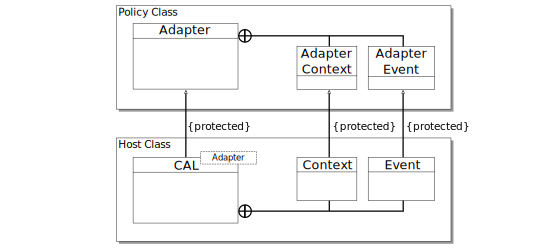
\includegraphics[width=\textwidth]{graphics/40_cal_uml}
    \caption{  }
    \label{fig:cal_uml}
  \end{figure}

  % Descrption Communication operations
  Usually, the adapter has to provide all communication and context
  operations. But, policy based design has the characteristic
  that if a member function not used through the host class, the
  compiler will not care if this function is implemented by the policy
  or not. Thus only the used member functions have to be implemented
  in an adapter (e.g just p2p functionality). But for sake of
  completeness an adapter should implement the whole policy interface.

  % Description Context + Event
  In addition to communication and context related member functions,
  the adapter has also to provide a inner context and a inner event
  class. Meaning and interface of these classes were explained in
  section \ref{sec:cal_comm}. Both contain the adapter specific
  implementations. The interface of these two inner classes is defined
  by according inner classes of the CAL and implanted by inheritance
  (Figure \ref{fig:cal_uml}.

\item The MPI Adapter as Reference Implementation

  The reference adapter implementation is based on MPI as existing
  communication layer.  MPI (Section \ref{sec:mpi}) was as choosen ,
  because it already brings a lot of functionality required by the CAL
  interface from the scratch. Additionally it is available on wide
  range of compute systems and can be used for free by open source
  implementations. To address MPI, the MPI C language binding is used
  inside the adapter. An alternative would be the boost::mpi c++
  implementation, which presupposes that beside a MPI implementation
  also the boost library is installed.

  Implementing the communication operation is straight forward, just a
  forwarding of arguments and a call to MPI. More tricky is the
  support of abitrary binary operations for the reduce operation and
  the support of abitrary data types of the trasmitted data.

  \begin{itemize}
  \item Binary Function

    The binary functions that takes the CAL as argument for reduce 
    operations have to be translated to binary MPI operations.

    There exists two possible ways to do so. The easiest way, is that
    the MPI adapter provides all binary MPI functions by itself as
    kind of a struct with static const expressions (Listing
    \ref{lst:mpi_bin}). The reduce operation handed over as
    BinaryOperations::MAX.

    \begin{lstlisting}[language=C++]
      struct BinaryOperations { 	
        static constexpr BinaryOperation MAX = MPI_MAX; 	
        static constexpr BinaryOperation MIN = MPI_MIN; 	
        static constexpr BinaryOperation SUM = MPI_SUM; 	
        static constexpr BinaryOperation PROD = MPI_PROD;
	...
      };
    \end{lstlisting}
    \label{lst:mpi_bin}

    The downside of the first approach is that only the predefined
    operations of MPI can be used. But it is possible to create
    abitrary binary functions with MPI\_Op\_create. This can be done
    for all handed over binary operation from the CAL. The only
    requirement is that the binary operation has to be a struct like
    discussed in section \ref{sec:cal_collective}.  Because of more
    flexibility the second approach was choosen to implemend binary
    functions for the MPI adapter.

  \item  Data Type Conversion 

    MPI predefines on one hand its primitive data types, but on the
    other hand also provides facilities to define own data structures
    based upon sequences of the MPI promitive data types. Such user
    defined structures are called derived data types. Primitive data
    types are contiguous. Derived data types allow you to specify
    non-contiguous data in a convenient manner and to treat it as
    though it was contiguous.

    The primitive c++ data types can be mapped directly to primitive
    C++ data types. The conversation is implemented by c++ traits .
    First, a generic template is defined that implements the default
    behaviour (Listing \ref{lst:mpi_trait1}). In this case unknown
    types will assumed to be MPI\_CHAR. The second template is a
    specialisation for int, which will be transformed to MPI\_INT
    (Listing \ref{lst:mpi_trait2}).


    \begin{lstlisting}[language=C++]
      template<typename T>
      struct MPIDatatypes{
	static constexpr MPI_Datatype type = MPI_CHAR;
      };
    \end{lstlisting}
    \label{lst:mpi_trait1}

    \begin{lstlisting}[language=C++]
      template<>
      struct MPIDatatypes<int>{
    	static constexpr MPI_Datatype type = MPI_INT;
      };

    \end{lstlisting}
    \label{lst:mpi_trait2}


    More complex data types (e.g structs or classes) have to be
    transformed into derived data types. This transformation is
    available in the boost::mpi implementation. Thus switching to
    boost::mpi \cite{ref:boost::mpi} would solve this problem without
    any further effort.

  \item MPI specific Context
  \item MPI specific Event
  \end{itemize}

\item Graph Based on the Boost Graph Library

  % BGL as backend
  The graph introduced in section \ref{sec:graph} was not written from
  the scratch. There are a varity of libraries providing graph
  implementations. Because of the closeness of the boost library to
  the C++ STL, the boost graph library \cite{ref:boost::bgl}, short
  BGL, was choosen. While the BGL provides a lot of functionality,
  just a small subset is really needed for the purposes of this
  library. Thus the BGL is wrapped inside a graph class just providing
  standard graph funcionality.

  \begin{itemize}  

  \item Vertices identified by Properties

    % Properties
    Like in section \ref{sec:graph} discussed, a graph has so called
    properties that can be used to describe its vertices and
    edges. The BGL itself refers to vertices by integer numbers,
    whereby properties of this integer vertices can be queried from so
    called property maps. Here the vertices and edges are represented
    by its property and are configured at compile time.  The
    properties are structs or classes with abitrary content. However
    the properties need to provide an id member variable to create an
    internal connection of vertices to properties.  Thus asking for
    the vertices of the graph, returns a vector of vertices. That
    vector is a list of vertex properties in the context of the BGL,
    whereby every property is connected by its id to the graph.
  
  \item Operations on the graph / vertices
    % Operations
    The graph provides simple graph operations like retrieving all
    vertices, retrieving adjacent vertices, retrieving in and out
    edges.
    \todo{Is there more Information needed? Because it is not that interesting}

  \item Creation of subgraphs
    % Subgraph Createion
    Another reason for the BGL is the builtin subgraph support. The
    creation of subgraphs is meant to be used as an equivalent to the
    creation of contexts in the CAL. Thus a subgraph can be created from its
    supergraph by a subset of its vertices. Collective operations on
    this subgraph only consider vertices within this subgraph.
  \end{itemize}

\item GraphCommunicator + NameService  

\item Configuration of an Application by Templates
  
  
  \begin{itemize}
  \item Creation of a Graph
  \item Example Configuration of a Communication System
  \end{itemize}

\item Implementing a Game of Life
  \begin{itemize}
  \item Based on Cells
  \item Based on Bundles
  \end{itemize}

\end{itemize}




\cleardoublepage

%%% Local Variables:
%%% TeX-master: "diplom"
%%% End:
